%%%%%%%%%%%%%%%%%%%%%%%%%%%%%%%%%%%%%%%%%%%%%%%%%%
\chapter{Toolkits}
%%%%%%%%%%%%%%%%%%%%%%%%%%%%%%%%%%%%%%%%%%%%%%%%%%

Las funciones que que aparecen en este capítulo no son necesariamente
parte de un toolkit de Matlab. No es más que una clasificación artificial
de las funciones con una finalidad concreta que no justifica la creación
de un capítulo a parte. Esta sección es mucho menos amplia de lo que
debería, se ha sacrificado a propósito a favor de temas más básicos
como el cálculo el álgebra o el dibujo de gráficas. Mientras todo
lo escrito hasta aquí es casi definitivo este capítulo no se considerará
nunca como terminado.


\section{Estadística descriptiva y análisis de datos}

Matlab es un lenguaje muy utilizado en análisis de datos, tanto
experimentales como producidos por otros programas. En el caso de las
series de datos experimentales habrá que importar un archivo
almacenado en un formato compatible y asignar todos los valores a una
variable; más adelante aprenderemos a hacerlo.

Supongamos el caso ideal de que ya tenemos todos los datos cargados en
una variable. Matlab tiene una cantidad enorme de rutinas que
facilitan el análisis de datos de modo interactivo. las funciones son
tan de alto nivel que es posible sacar cualquier resultado secundario
sin necesidad de pensar un script; directamente con la consola. las
funciones más útiles son:

\begin{description}
\item [mean\index{mean}]Calcula la media de una muestra de datos:
  $\bar{x}=\frac{1}{n}\sum_{n=1}^{n}x_{i}$.
\item [std\index{std}]Calcula la desviación típica de una muestra de
  datos: $s=\sqrt{\frac{1}{n-1}\sum_{i=1}^{n}(x_{i}-\bar{x})^{2}}$.
\item [median\index{median}]Calcula la mediana de la muestra.
\item [min\index{min}]Valor mínimo de la muestra.
\item [max\index{max}]Valor máximo de la muestra.
\item [sort\index{sort}]Ordena los elementos de menor a mayor.
\item [center\texttt{\index{center}}]Resta el valor medio de la serie
  de datos.
\end{description}

\subsection{Ajuste de curvas por mínimos cuadrados.}

Supongamos que tenemos una serie de datos obtenidos mediante un
experimento y queremos hacer cálculos con ellos. El principal
impedimento es que ya no disponemos de una serie continua de datos
sino de medidas discretas.  Las dificultades que se presentan son
numerosas; no podemos poner dichos datos en un sistema de ecuaciones
no lineales porque no es diferenciable, tampoco en una ecuación
diferencial. La solución es convertir estos datos en una muestra
contínua que nuestras herramientas numéricas puedan manejar.

La práctica más común es la de utilizar un ajuste polinómico. El
polinomio resultante se obtiene resolviendo el problema de mínimos
cuadrados.  El grado del polinomio es uno de los datos que debemos
escoger. Suele ser una regla válida que polinomios de mayor órden
consiguen menor error pero no es siempre cierta. \textbf{Es bastante
  usual utilizar erroneamente el ajuste por mínimos cuadrados; sirven
  para crear un modelo polinómico de una función, no para conseguir
  una curva a través de unos puntos; para esto está la interpolación.}
Por ejemplo, supongamos que disponemos de la siguiente serie de datos:

\begin{center}\begin{tabular}{|c|c|}
    \hline 
    x&
    y\tabularnewline
    \hline
    \hline 
    0&
    2.0000\tabularnewline
    \hline 
    0.1&
    2.1850\tabularnewline
    \hline 
    0.2&
    2.2011\tabularnewline
    \hline 
    0.3&
    2.5762\tabularnewline
    \hline 
    0.4&
    2.5780\tabularnewline
    \hline 
    0.5&
    2.9711\tabularnewline
    \hline 
    0.6&
    2.7816\tabularnewline
    \hline 
    0.7&
    3.0766\tabularnewline
    \hline 
    0.8&
    2.8277\tabularnewline
    \hline 
    0.9&
    3.6763\tabularnewline
    \hline 
    1&
    3.6933\tabularnewline
    \hline
  \end{tabular}\end{center}

\begin{description}
\item [polyfit\texttt{\index{polyfit}}]Devuelve los coeficientes del
  polinomio del grado que queramos y soluciona el problema de ajuste
  por mínimos cuadrados.
\end{description}
Introducimos ahora las dos series de datos e intentamos ajustarlo por
mínimos cuadrados para crear un modelo \textbf{lineal} de los datos
adquiridos. Lo conseguimos con la siguiente líneas de código:

\begin{verbatim}
fit=polyfit(linspace(0,1,11),y,1)
fit=
  1.5928
  1.9828
\end{verbatim}
Ahora tenemos dos números en un vector llamado \texttt{fit}, este
vector son los dos coeficientes del polinomio que ajusta los datos;
una recta. Ahora representaremos gráficamente los datos del siguiente
modo

\begin{verbatim}
plot(linspace(0,1,11),y,'b*')
hold on
plot(linspace(0,1,11),polyval(fit,linspace(0,1,11)))
\end{verbatim}
El resultado es la figura \ref{cap:Ajuste por minimos cuadrados}

%
\begin{figure}[h]
  \centering{}

  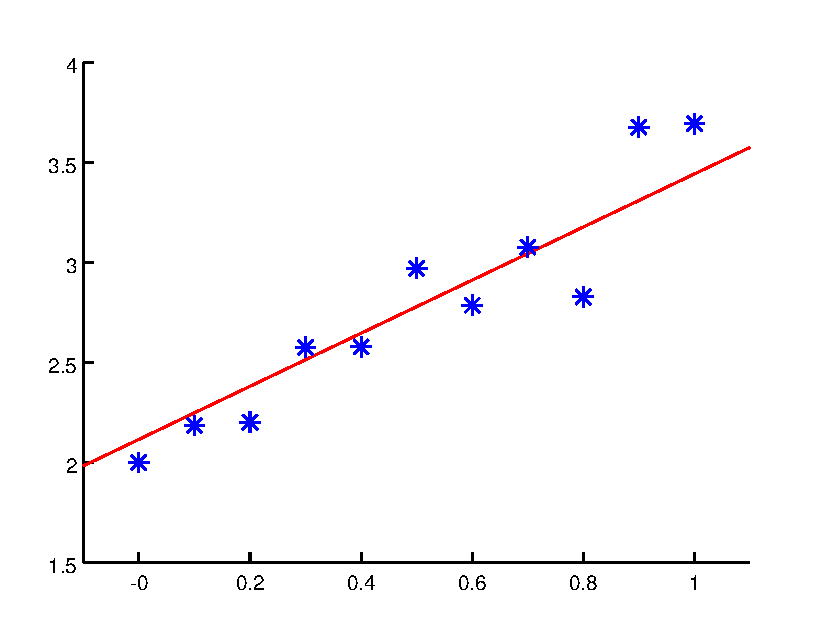
\includegraphics[%
  width=10cm,
  height=12cm,
  keepaspectratio]{figuras/fitting}


\caption{\label{cap:Ajuste por minimos cuadrados}Ajuste por mínimos cuadrados
de una serie de puntos}
\end{figure}


Resolver un problema de mínimos cuadrados es en el fondo resolver
un problema mal condicionado. Si se plantean las ecuaciones del problema
llegamos a un sistema lineal mal condicionado. El criterio de resolución
suele ser el de minimizar el error cuadrático de la solución dada
(por eso el nombre de mínimos cuadrados). Este es exactamente el mismo
problema planteado en la pseudoinversa, operación que también se realiza
por mínimos cuadrados.

Nada nos obliga a ajustar los datos mediante un polinomio; la condición
de minimización del error cuadrático puede utilizarse con cualquier
función aunque siempre será más sencillo hacerlo con polinomios. Una
práctica muy habitual es utilizar un ajuste exponencial, táctica para
la que Matlab no ha escrito ninguna función. El motivo es bien sencillo,
si tenemos una nube de puntos que creemos sigue un modelo exponencial
lo único que debemos hacer es calcular el logaritmo de la serie de
datos para lo que recuperaremos automáticamente el ajuste polinómico.


\subsubsection{¿Qué calcula el ajuste polinómico por mínimos cuadrados?
  \label{sub:=BFQu=E9-calcula-el}}

Cuando hemos hablado de mínimos cuadrados en realidad nos referimos a
los Mínimos Cuadrados Lineales Generales. El problema planteado es el
de ajustar una serie de datos cualquiera a una función de la forma:

$$
y(x)=a_{1}+a_{2}x+a_{3}x^{2}+\ldots+a_{N}x^{N-1}$$

Este no es más que el tipo más sencillo de ajuste. Podríamos utilizar
también series de funciones armónicas o funciones arbitrarias de la
forma

$$
y(x)=\sum_{k=1}^{N}a_{k}X_{k}(x)$$

en las que $X$ representa una base de funciones. El objetivo es
minimizar el funcional error representado por la expresión

$$
\chi^{2}=\sum_{i=1}^{N}\left[
  \frac{y_{i}-\sum_{k=1}^{N}a_{k}X_{k}(x_{i})}{\sigma_{i}}\right]^{2}
$$

donde $\sigma$ es la desviación estándar de la muestra i-ésima. Esta
formulación permite generar una matriz para una aplicación lineal:

$$
A_{ij}=\frac{X_{j}(x_{i})}{\sigma_{i}}$$

Matriz que posee muchas más filas que columnas. La buena noticia es
que acabamos de generar un problema tan simple como una aplicación
lineal ($\mathbf{a}x=b$), la mala es que la matriz no es cuadrada y no
servirán los métodos de resolución convencionales. Una de las posibles
estrategias de resolución es utilizar una SVD para resolver el
sistema.

\section{Interpolación y aproximación de funciones}

La aproximación local o global de funciones es una parte esencial del
cálculo y del análisis.  Esta sección supone que ya conocemos los
desarrollos de Taylor o las transformadas de Fourier.  Algunos de los
métodos planteados no son más que la extensión discreta de métodos
comunes.

Aunque no sea del todo riguroso dividiremos este tema en tres partes
según las características del desarrollo de nuestros datos.  En
cálculo numérico siempre nos veremos obligados a describir una función
de un modo discreto, ya sea por el valor que toman en algunos puntos o
por los coeficientes de un desarrollo.  Dichas descripciones son más o
menos adecuadas según la finalidad que busquemos.

Hablaremos de la interpolación polinómica a trozos cuando sean dados
los valores de la función en unos puntos o nodos fijos.  Utilizaremos
funciones sencillas para intentar hallar una función continua que pase
por todos los puntos.  Hablaremos de interpolación polinómica cuando
queramos modelar una función conocida o desconocida mediante funciones
más simples buscando el mínimo error posible.  Se diferencia de la
anterior en que nuestro dato es una función y no una serie de puntos,
esto nos permitirá escoger los nodos para buscar el mínimo error de
interpolación.  Por último trataremos a parte los desarrollos en serie
de funciones sea cual sea la base (funciones armónicas, polinomios)

En el primer caso buscaremos convertir unos datos de naturaleza
discreta en una función continua, en el segundo y el tercer caso
intentaremos describir una función de un modo discreto, ya sea por sus
valores o por unos coeficientes, por ejemplo para hallarla cuando es
el resultado de una ecuación en derivadas parciales.

Los métodos numéricos no son exclusivos de cada uno de los objetivos,
los splines, por ejemplo, sirven tanto para hallar una curva contínua
como para describir una función mediante unos coeficientes.  El uso de
estas distinciones es que Matlab se basa más en la utilidad del método
numérico que en su naturaleza.  Si queremos splines para interpolar
utilizaremos una función distinta de la dedicada a hallar sus
coeficientes.

\subsection{Interpolación polinómica a trozos}

La interpolación polinómica a trozos será \emph{para nosotros} la
técnica de hallar una curva que pase por unos puntos dados.  Se dice
que es a trozos porque se utilizan polinomios de bajo orden definidos
a intervalos.

\begin{description}
\item [interp1\texttt{\index{interp1}}]Usa los puntos para interpolar
  en una dimension. Soprota interpolación discreta, lineal, cúbica,
  hermitiana y por splines cúbicos.
\end{description}
Un ejemplo gráfico es el siguiente script:

\begin{verbatim}
xf=0:0.05:10;yf=sin(2*pi*xf/5);
xp=0:10 ;yp=sin(2*pi*xp/5);
lin=interp1(xp,yp,xf);
spl=interp1(xp,yp,xf,'spline');
cub=interp1(xp,yp,xf,'cubic');
near=interp1(xp,yp,xf,'nearest');
title('Comparacion de las opciones de interp1')
plot(xf,yf,xf,lin,xf,spl,xf,cub,xf,near)
legend('real','lineal','splines','cubica','discreta')
\end{verbatim}
Cuyo resultado es la figura \ref{cap:Comparaci=F3n-de-los}.

%
\begin{figure}[h]
  \centering{}

  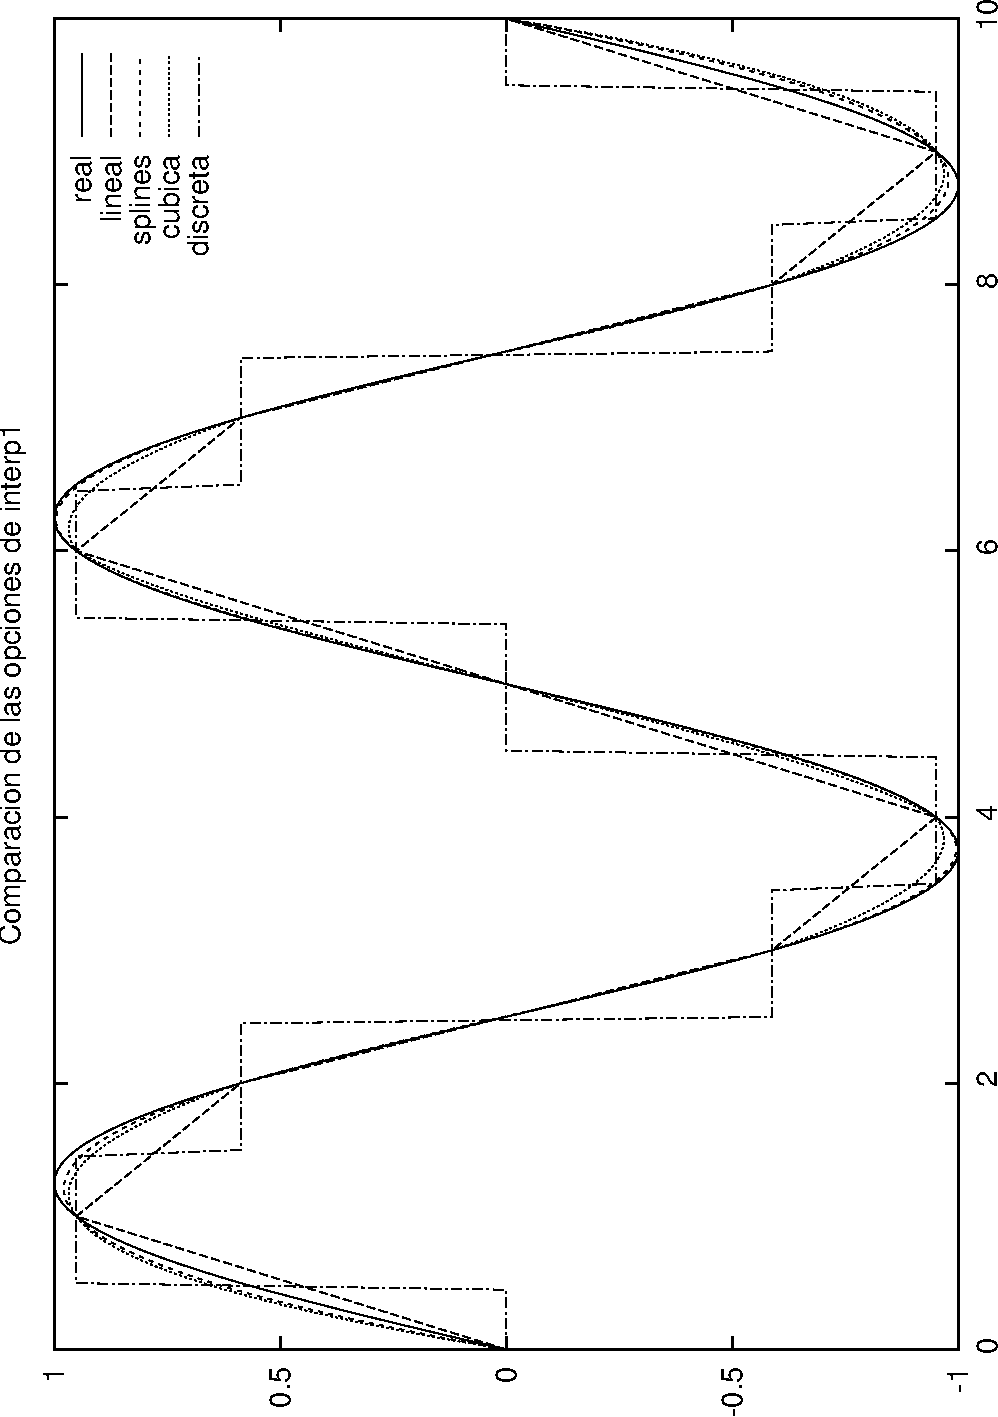
\includegraphics[%
  width=12cm,
  height=12cm,
  keepaspectratio]{figuras/figuraejemplo2}


  \caption{\label{cap:Comparaci=F3n-de-los} Comparación de los métodos
    de interpolación}
\end{figure}


\begin{description}
\item [interp2\texttt{\index{interp2}}]Interpolación polinómica
  bidimensional.
\end{description}
De entre todos los métodos de interpolación a trozos el más efectivo
suele ser siempre el uso de splines. Un spline es una curva cúbica; de
este modo reduciremos en gran medida el error en el caso que los
puntos \emph{sean de una función suave}, cosa que no sabemos. Cuando
interpolamos por trozos es importante conocer algo de información
sobre la función que representan, no sirve ninguna formula universal

Sería muy lógico en este punto plantearse la siguiente pregunta. ¿Por
qué escoger una función definida a intervalos y no un único polinomio
de grado igual al número de puntos menos 1? La respuesta aparece
cuando intentamos realizar el cálculo. Los polinomios de alto orden
tienen tendencia a oscilar en sus extremos, es el llamado fenómeno de
Runge.  Como patrón diremos que todo lo relacionado con polinomios de
alto orden suele acarrear problemas. Trataremos con más profundidad la
interpolación polinómica en un dominio finito en la sección
\ref{sub:Aproximación-de-funciones}.

\subsubsection{Splines}
\label{sec:splines}
La interpolación polinómica a trozos más común en Matlab es la
interpolación mediante splines.  Un spline es una curva definida
mediante polinomios en intervalos finitos, la interpolación será
entonces del orden que deseemos según el polinomio aunque lo más
frecuente será utilizar splines cúbicos.  Como en muchos otros casos
los splines no sirven únicamente para convertir en continua una serie
de datos discreta, función que cumple \texttt{interp1}.  Pueden servir
también para analizar más profundamente los datos estimando sus
derivadas e incluso para resolver ecuaciones en derivadas parciales.

Para quien desee algo de rigor matemático definimos un spline como el
conjunto de polinomios $p_j(x)$ que ajustan una determinada función
$f(x)$ en $[a,b]$, donde cada polinomio tiene validez en un intervalo
$\xi_j \in [a,b]$.  Además de imponer que la curva pase por todos los
puntos podemos imponer también que dichos polinomios se unan
suavemente al final de sus intervalos de definición.  Podemos
representar el conjunto mediante sus coeficientes y los nodos (
\emph{pp form})

$$p_j(x)=\sum_{i=1}^k(x-\xi_j)^{k-i}c_{ij}$$

o como B-spline, generalización de las curvas de Bézier.

Matlab, en su \emph{spline toolkit}, proporciona funiones para
calcular y evaluar con toda libertad los coeficientes de una
interpolación a trozos mediante splines, \emph{piecewise spline
  interpolation}.  Algunas de las funciones disponibles son las
siguientes:

\begin{description}
\item[spline\index{spline}] Llamada con dos parámetros retorna la
  matriz de coeficientes de la interpolación.  Llamada con tres
  parámetros retorna el valor de la interpolación en los valores
  dados.
\item[ppval\index{ppval}] Evalúa la interpolación mediante splines en
  los puntos dados dada su representación en coeficientes.
\item[csapi\index{csapi}] Define
\item[csape\index{csape}] Define
\end{description}

Un posible uso de los splines es la interpolación de curvas en más de
una dimensión.  Es un método muy habitual en diseño y es la base de
las herramientas de CAD con las NURBS (Non-Uniform Rational B-Splines).
Mediante puntos de control y unas pocas transformaciones geométricas
los splines definen casi todas las piezas producidas industrialmente.

\subsubsection{Regeneración de funciones mediante datos discretos}

Como ya hemos mencionado con anterioridad, uno de los problemas de
tratar con series discretas de datos es precisamente su no
continuidad.  Hay varias maneras de pasar los datos a una función y
hemos analizado que el ajuste polinómico no siempre es una buena
opción. Una solución más o menos universal es la de crear una función
mediante una interpolación y un function handle. Para ello sólo
tenemos que definir las series de datos y pasarlos como argumento a la
vez que definimos una variable independiente adicional. Por ejemplo,
suponemos que tenemos la siguiente serie de datos:

\begin{verbatim}
x=[1 2 3 4 5 6 7 8]
y=[2 4 3 5 4 6 5 7]
\end{verbatim}
Y queremos generar una función que sea capaz de proporcionar los datos
de forma continua. La solución es la creación del siguiente function
handle:

\begin{verbatim}
>> newfunc=@(z) interp1d([1 2 3 4 5 6 7 8],...
    [2 4 3 5 4 6 5 7],z,'spline');
\end{verbatim}

A todos los efectos esto es una nueva función que pasa por todas las
parejas de puntos $(x,y)$:

\begin{verbatim}
>> newfunc(3.443)
ans = 3.9162
\end{verbatim}

La técnica de reducir variables mediante function handles no es válida
en Octave, donde los FH son estrictamente funciones independientes.


\subsection{Transformadas rápidas de Fourier}

Un desarrollo posible de una función \textbf{periodica} es el
desarrollo de Fourier. En él las funciones ortogonales que nos sirven
de base son funciones armónicas que llamaremos $\Phi_{k}$. El
desarrollo de la función $u$ es entonces:
$$u=\sum_{k=-\infty}^{k=\infty}\hat{u}\Phi_{k}.$$ donde $\hat{u}$ son
los coeficientes de Fourier que \textbf{suelen ser números complejos}.
Si la función admite el desarrollo anterior también admitirá una
\emph{serie truncada de fourier}. Esta serie tiene la forma:
$$P_{N}u=\sum_{k=-\frac{N}{2}}^{k=\frac{N}{2}-1}\hat{u}_{k}e^{ikx}$$
que constituye la serie truncada de Fourier de orden $N$. Los
coeficientes se calculan exactamente del mismo modo que la anterior
con la diferencia que truncamos el desarrollo a partir de un cierto
número de onda.  En el cálculo numérico nunca trabajaremos con
desarrollos con una cantidad infinita de términos; esto es dominio del
cálculo simbólico.

Si aproximamos la función inicial por un polinomio interpolante
definido a partir de una serie de puntos llegamos a la \emph{serie
  discreta de Fourier}. Se dice discreta porque tiene como datos los
puntos en los que se evalúe la función. Exactamente del mismo modo
podríamos estar trabajando con una serie de puntos experimentales.
Esto generará un desarrollo discreto porque sólo con unos cuantos
puntos no tenemos suficiente información como para llegar a una serie
infinita.

Como estamos obteniendo toda la información posible normalmente se
habla de \emph{transformada discreta de Fourier}. El algoritmo para
calcularla es la \emph{t}ansformada \emph{rápida de Fourier} o
\emph{Fast Fourier Transform} (FFT).

\begin{description}
\item [fft\texttt{\index{fft}}]Aplica la transformada rápida de
  Fourier a una serie de puntos utilizando como funciones base
  $\Phi_{x}(x)=e^{ikx}$.
\item [ifft\index{ifft}]Calcula la antitransformada rápida de Fourier.
\end{description}
Las fft's se usan muchísimo en los métodos espectrales, resolución de
ecuaciones en derivadas parciales lineales y no lineales, análisis de
datos y filtrado de señales. Muchos de los problemas de la física con
condiciones de contorno periodicas son mucho más sencillos en su
formulación espectral.%
\footnote{La gran ventaja de las transformadas rápidas de Fourier es
  que son una operación especialmente rápida cuando tenemos series de
  $2^{n}$ puntos. En estos casos se hacen del órden de $N\log N$
  operaciones para calcularla. Esto las hace muy útiles en la
  resolución de ecuaciones en derivadas parciales lineales (ecuación
  de ondas) o por métodos espectrales. Un caso especialmente
  importante es el de la ecuación de Poisson
  ($\nabla^{2}\phi=f(\vec{x})$).

  Supongamos que tenemos las ecuaciones de Navier-Stokes en dos
  dimensiones.  Se demuestra que se pueden reescribir en función de
  $\omega$ y de $\psi$, la vorticidad y la función de corriente de la
  siguiente manera:
$$ \frac{\partial\omega}{\partial
  t}+\frac{\partial\omega}{\partial x}\frac{\partial\psi}{\partial
  y}-\frac{\partial\omega}{\partial y}\frac{\partial\psi}{\partial
  x}=\frac{1}{Re}\nabla^{2}\omega$$
  $$
  \nabla^{2}\psi=-\omega$$ Imaginemos entonces que queremos resolver
  un problema de turbulencia 2D isótropa con condiciones de contorno
  periódicas. Esto nos obliga a resolver una ecuación de Poisson por
  cada paso temporal, operación bastante costosa porque requiere la
  inversión de una matriz. Podemos ahorrarnos gran cantidad de
  operaciones si hacemos la transformada de Fourier de la segunda
  ecuación:$$
  \frac{\partial^{2}\hat{\psi}(i,j)\exp(\imath(kx+ly))}{\partial
    x^{2}}+\frac{\partial^{2}\hat{\psi}(i,j)\exp(\imath(kx+ly))}{\partial
    y^{2}}=-\hat{\omega}\exp(\imath(kx+ly))$$
  $$
  \hat{\psi}(i,j)(k^{2}+l^{2})=\hat{\omega}(i,j)$$ Que es un sistema
  de ecuaciones de resolución trivial. Acto seguido hacemos la
  antitransformada de los coeficientes $\hat{\psi}(i,j)$ y ya podemos
  pasar al paso de la ecuación parabólica.%
}

Disponemos también de otras funciones que encapulan tareas comunes en
las que están involucradas transformadas de fourier

\begin{description}
\item [fftshift\index{fftshift}]Mueve el primer número de onda
  (frecuencia cero) al centro del espectro.
\item [fftfilt\index{fftfilt}]Aplica directamente un filtro espectral.
\item [fft2\index{fft2}]Transformada rápida de Fourier bidimensional.
  También disponemos de una antitransformada para esta función
\item [fftn\index{fftn}]Transformada rápida de Fourier n-dimensional.
  Existe \texttt{ifftn}.
\end{description}
Las librerías de transformadas rápidas de Fourier suelen disponer de
transformadas del seno y del coseno para cubrir los casos de
condiciones de contorno no periodicas. Los drivers para estas
bibliotecas no son tan completos en Matlab y tendremos que convertir
la transformada exponencial en transformada de seno o de coseno
manualmente.


\subsection{Aproximación de
  funciones\label{sub:Aproximación-de-funciones}}

Esta técnica, aunque coceptualmente muy parecida a la interpolación
polinómica a trozos, suele tener usos completamente distintos. La
aproximación de una función o de una serie de puntos por un único
polinomio en un dominio dado se acerca más al desarrollo en serie de
Fourier que a la interpolación polinómica a trozos. Los polinomios de
Lagrange, de Legendre o de Chebyshev fueron creados para desarrollar
funciones continuas en dominios finitos mediante una base polinómica.
Tienen un uso esencial en la evaluación de funciones complejas en
dominios finitos y en los métodos espectrales de resolución de
ecuaciones en derivadas parciales.

La interpolación polinómica no suele utilizarse para ajustar una serie
de puntos dados por culpa del fenómeno de Runge. Supongamos que
tenemos la siguiente serie de puntos $y$ en función otra serie
equiespaciada de puntos $x$.

\begin{verbatim}
x =
 Columns 1 through 8:
 -1.00000  -0.87500  -0.75000  -0.62500  -0.50000  -0.37500  -0.25000  -0.12500
 Columns 9 through 16:
  0.00000   0.12500   0.25000   0.37500   0.50000   0.62500   0.75000   0.87500
 Column 17:
  1.00000
y =
 Columns 1 through 8:
 0.058824  0.075472  0.100000  0.137931  0.200000  0.307692  0.500000  0.800000
 Columns 9 through 16:
 1.000000  0.800000  0.500000  0.307692  0.200000  0.137931  0.100000  0.075472
 Column 17:
 0.058824
\end{verbatim}
Supongamos ahora que queremos ajustarla por un polinomio de grado
$N-1$ suponiendo $N$ el número de puntos de la serie. El polinomio
será entonces:
$$ p(x)=\sum_{i}^{N}a_{i}x^{i-1}$$
problema que se cerrará con la condición de que $p(x_{i})=y_{i}$.  Al
final se llega a la misma ecuación de siempre:\[ Ac=y\] donde $A$ es
la matriz de Vandermonde generada con los puntos $x_{i}$, $c$ el
vector de incógnitas de los coeficientes y $y$ el vector de puntos de
la serie $y_{i}$. El vector de coeficientes se genera con este código:

\begin{verbatim}
>> c=vander(x) \y'
c =
    6.4739e+03
    3.6848e-11
   -2.1040e+04
   -1.0123e-10
    2.7271e+04
    1.0430e-10
   -1.8231e+04
   -5.0934e-11
    6.8268e+03
    1.2373e-11
   -1.4741e+03
   -1.4184e-12
    1.8795e+02
    6.5051e-14
   -1.5402e+01
   -8.4500e-16
    1.0000e+00
\end{verbatim}
Si representamos este polinomio de orden 16 con los puntos que tiene
interpolar junto con la función solución
$y(x)=\frac{1}{1+16x^{2}}$(figura \ref{cap:runge}):

%
\begin{figure}[h]
  \centering{}

  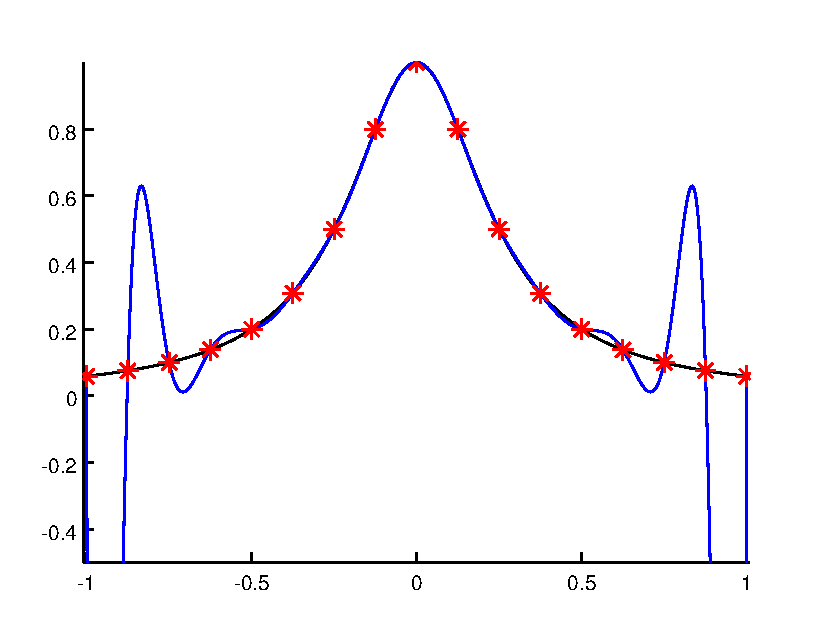
\includegraphics[%
  width=10cm,
  height=12cm,
  keepaspectratio]{figuras/interpeq}


  \caption{\label{cap:runge}Demostración del fenómeno de Runge}
\end{figure}


Como vemos, la función interpolante cumple los requisitos impuestos,
pasa por todos los puntos; pero no hace nada más bien. ¿Cuál es
entonces el problema? ¿Qué hay que hacer para solucionarlo? La
interpolación polinómica es un problema global, es decir, intenta
aproximar toda una función con una cantidad limitada de datos (los
puntos de los que tenemos valores). A la función interpolante los
árboles no le dejan ver el bosque, si quiere ajustar con unos puntos
dados (nodos) es incapaz de capturar la función de la que provienen.

La solución es comprender las implicaciones globales del problema.  Ya
no estamos intentando hacer pasar una curva por una serie de puntos,
estamos intentando resolver la aproximación de la misma curva. La
solución la encontramos desde el punto de vista global... ¿Por qué los
nodos deben ser equiespaciados? ¿Y si acercamos los nodos entre ellos
(clustering) en las zonas donde los errores son más elvados?  Sean
cuales sean los tipos de polinomios que utilicemos así como el orden
del que sean hay nodos más adecuados para minimizar el error del
problema global, por ejemplo los nodos de Chebyshev de la forma:
$$x_{j}=cos(j\pi/N),\qquad j=0,1,...,N$$
puntos de Chabyshev-Lobatto o puntos extremos de Chebyshev. Esta
formula es la proyección de los puntos equiespaciados en una
circunferencia de radio unidad en el eje de abcisas. Si ahora en vez
utilizar los nodos equiespaciados utilizamos los nodos óptimos de
Chebyshev llegamos a que el polinomio de interpolación es
sensiblemente mejor (figura \ref{cap:chebyshev}):

%
\begin{figure}[h]
  \centering{}

  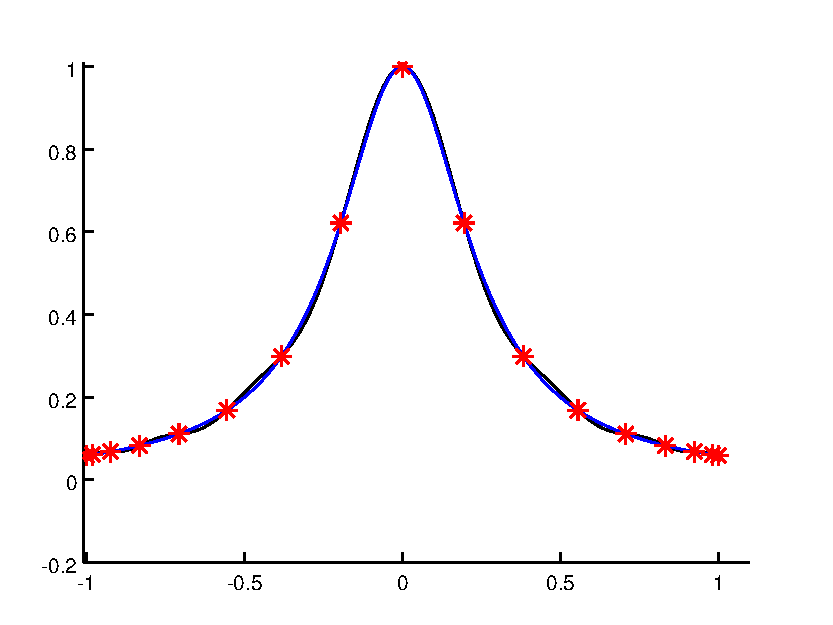
\includegraphics[%
  width=10cm,
  height=12cm,
  keepaspectratio]{figuras/chebyshevnodes}


  \caption{\label{cap:chebyshev}Uso de los nodos óptimos de Chebyshev
    para reducir el error de interpolación}
\end{figure}


Vemos entonces que recurrir a una elección óptima de nodos permite
utilizar polinomios como base de desarrollos de funciones con un error
más que aceptable con todas las ventajas que implica trabajar con
polinomios en nuestros cálculos.

\begin{description}
\item [Importante:]La interpolación polinómica es un problema global.
  No depende únicamente del número de puntos sino de su elección.
\end{description}
Una demostración de hasta dónde llega la importancia de elegir bien
los nodos es pensar que el error que se comete con un polinomio de
grado mayor no necesariamente se reduce con lo que estamos malgastando
tiempo y potencia de cálculo sin ganar precisión. Hay que hacer las
cosas con cuidado.


\section{Resolución de ecuaciones no lineales y optimización.}

Este apartado merece un pequeño comentario de entrada. Matlab posee
una más que amplia selección de funciones orientadas a la
optimización.  Matlab contiene funciones para hacer casi todo lo
imaginable como buscar ceros de funciones n-dimensionales y no
lineales, mínimos de funciones condicionados, programación
cuadrática... El gran problema es que todas estas herramientas están
en un toolkit que no forma parte de la instalación básica del
programa. En el caso que estemos delante de una versión comercial o de
estudiante del Matlab es posible que no dispongamos de ninguna de las
funciones anteriormente mencionadas.

No tiene mucho sentido entrar los detalles del Optimization Toolkit
porque la ayuda en formato HTML que se incluye en el paquete es más
que suficiente. Se podría decir que es una buena introducción a la
optimización en general.

Este tema es difícil de encajar en el planteamiento general del libro.
Siempre hemos buscado un planteamiento agnóstico respecto a los dos
intérpretes muy difícil de mantener en este caso. Octave sólo contiene
las funciones básicas de optimización, la colección es pobre si se
compara con el Optimization Toolkit; pero en la mayoría de los casos
es más que suficiente.

Veremos entonces sólo una introducción básica a la optimización,
minimización de funciones, programación lineal y no lineal y búsqueda
de raíces de sistemas de ecuaciones no lineales.


\subsection{Resolución de ecuaciones no lineales. Root finding.}

La resolución de sistemas de ecuaciones no lineales podría
considerarse como una disciplina independiente de la optimización.
Algunos de los métodos de resolución no tienen absolutamente nada que
ver con los algoritmos de minimización de funciones. Sin embargo hemos
decidido mantener un órden consistente con el de los paquetes de
funciones de Matlab.

Root finding es el término inglés para la práctica de la resolución de
una ecuación que no tiene una solución analítica o con una solución
exacta demasiado costosa de encontrar. Fue uno de los primeros casos
en los que se aplicó el cálculo numérico porque es donde se hace
imprescindible.

Todos los métodos se basan en la aproximación mediante un desarrollo
en serie de la función en un punto inicial. Lo que los diferencia es
el tipo de desarrollo y cómo aproximan la función en el punto.  El
método más básico de todos es el método de \emph{Newton} que se basa
en la aproximación lineal de la función en cada punto para obtener la
siguiente raíz para iterar. El método de la secante no es más que una
aproximación grosera de la derivada mediante dos puntos. Luego nos
encontramos con los métodos \emph{Regula-falsi}, \emph{Ridders}...  o
más sofisticados como el \emph{Van Wijngaarden-Dekker-Brent}.

Todos los métodos se usan de la misma manera, se les da una función,
un punto inicial y se cruzan los dedos. Lo único que debemos saber del
\emph{Root finding} en Matlab es que todo lo lleva la función...

\begin{description}
\item [fzero\index{fzero}]Busca la solución más cercana al punto
  inicial dado de cualquier ecuación dada.
\end{description}
Lo único que debemos recordar es que como cualquier función a la que
hay que dar otra función como argumento nos obligará a utilizar un
function handle. Por ejemplo, queremos encontrar el cero de la
siguiente ecuación:
$$ \ln x-\sin x=0$$
Esta ecuación no tiene una solución analítica con lo que el uso del
cálculo numérico se hace imprescindible. Suele ayudar representar
gráficamente las dos funciones (figura
\ref{cap:Representación}) para saber si se cruzan en algún
punto; si buscamos una solución inexistente es probable que el método
nos devuelva soluciones complejas o espúreas.

%
\begin{figure}[h]
  \centering{}

  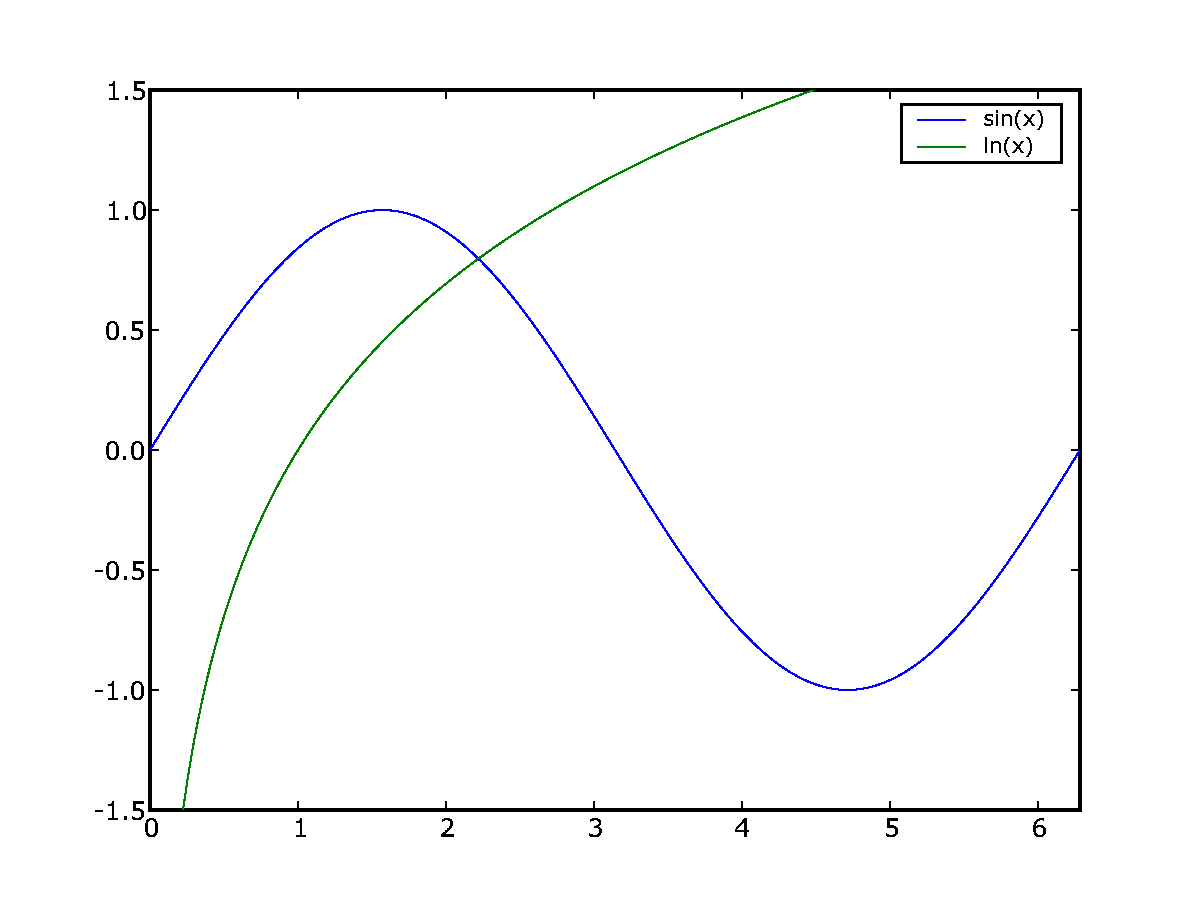
\includegraphics[%
  width=12cm,
  keepaspectratio]{figuras/fzero}


  \caption{\label{cap:Representación}Representación de las
    funciones a resolver.}
\end{figure}


La función que se resolverá será siempre de la forma $f(x)=0$, de modo
que nuestro function handle será:

  \begin{verbatim}
>> eq=@(x) log(x)-sin(x);
>> sol=fzero(eq,1);
>> sol
sol =
    2.2191 
\end{verbatim}
que es consistente con la solución intuida basándonos en la gráfica.

Una más que buena práctica es pedir una solución dentro de un
intervalo puesto que en muchos casos las ecuaciones no lineales pueden
tener varias e incluso infinitas soluciones. Sólo hay que cambiar el
punto inicial de iteración por un intervalo de búsqueda:

  \begin{verbatim}
>> eq=@(x) log(x)-sin(x);
>> sol=fzero(eq,[1 4]);
>> sol
sol =
    2.2191 
\end{verbatim}

\subsubsection{Más incompatibilidades entre Matlab y Octave.}

En la versión 2.1 de Octave el soporte para los function handles es
bastante limitado. Muchas de las funciones, sobretodo las que no son
más que llamadas a rutinas en fortran o C, deben obtener las funciones
por su nombre y no mediante un function handle. La función
\texttt{fzer}o en Octave es una víctima bastante desafortunada de esta
limitación.  Si intentamos resolver la ecuación anterior por el primer
método propuesto recibiremos un error, a priori incomprensible,
mientras que con el segundo script llegaremos a la solución.

El motivo es el exótico comportamiento de \texttt{fsolve} en Octave.
Si le pasamos sólo un parámetro, \texttt{fzero} llamará a la función
\texttt{fsolve} de la que hablaremos en el siguiente apartado.
\texttt{fsolve} no tiene soporte para function handles de modo que
tendremos que pasarle la función por su nombre despues de haberla
definido, por ejemplo:

  \begin{verbatim}
>> function y=eq(x)
... y=log(x)-sin(x);
... end
>> fzero('eq',1)

ans = 2.2191
\end{verbatim}
Tampoco es una gran dificultad añadida ya que Octave soporta la
definición de funciones mediante el intérprete a diferencia de Matlab.
En cambio, si definimos un intervalo de búsqueda de soluciones sí le
podremos pasar un function handle como argumento porque usa un método
de resolución alternativo%
\footnote{\texttt{fsolve} utiliza el método Powell mientras que
  \texttt{fzero} utiliza un método Brent.%
}:

  \begin{verbatim}
>> eq1=@(x) log(x)-sin(x);
>> fzero(eq1,[1,4])
ans = 2.2191 
\end{verbatim}

\subsection{Búsqueda de soluciones de sistemas de ecuaciones no
  lineales.}

Se define como solución de un sistema de ecuaciones como la $x$ que
cumple:\[ \mathbf{f}(x)=0\] siendo $\mathbf{f}$ la función vectorial
representa al sistema.

El objetivo de la búsqueda de soluciones de sistemas de ecuaciones no
lineales es siempre el mismo. Llegar a una solución válida del sistema
con el mínimo coste computacional posible. La no linealidad de las
ecuaciones puede provocar todo tipo de catástrofes como la no
convergencia o que el error se dispare hacia el infinito. Siempre se
parará automáticamente la iteración y se nos dará un mensaje de error.
El coste computacional es una complicación menor. Depende de dos
aspectos, la elección del punto inicial y el algoritmo de evaluación
del gradiente de la función.

Los métodos más sencillos de resolución de ecuaciones no lineales se
basan en la aproximación lineal de la función en un punto. Si hacemos
el desarrollo de Taylor de primer orden en el punto inicial tenemos
que:$$ \mathbf{f}(x)=\mathbf{f}(x_{0})+(x-x_{0})\mathbf{J}(x_{0})$$

fórmula a la que le siguen términos de mayor órden.
$\mathbf{J}(x_{0})$ es el gradiente de la función evaluado en el punto
$x_{0}$. Si suponemos que el resultado de la aproximación es la
verdadera raíz de nuestra función:
$$
\mathbf{f}(x_{0})+(x-x_{0})\mathbf{J}(x_{o})=0$$ obtendremos el
siguiente punto de la iteración, en este caso $x=x_{1}$:
$$x_{1}=x_{0}-\mathbf{J}^{-1}(x_{0})\mathbf{f}(x_{0})$$


Iteración que se llevará a cabo hasta que se una norma de la solución
sobrepase una cota de error. Este método es conocido como
\emph{Newton-raphson}.  Esto nos recuerda que una de las operaciones
con mayor coste computacional es precisamente la inversión de una
matriz. Además la matriz es el gradiente de la función en un punto,
gradiente que puede ser en algunos casos casi imposible de calcular.
Nos encontramos ante el problema de evaluar de una manera óptima un
gradiente para luego evaluarlo e invertirlo. Todo esto considerando
que el punto inicial nos lleve más o menos directamente a la solución
que buscamos.

Nada de esto debe hacernos perder la referencia de que lo realmente
importante de los métodos de resolución es la facilidad con la que
converjan a una solución más que la rapidez con que lo hagan. Al igual
que en el caso unidimensional, Matlab apuesta por la simplicidad.  La
función que nos realizará la tarea es:

\begin{description}
\item [fsolve\index{fsolve}]Busca una solución de un sistema de
  ecuaciones dado. Esta función es diferente según se use en Matlab o
  en Octave; la versión de Matlab llamará al sistema de ecuaciones
  mediante su nombre o con un function handle mientras que la versión
  de Octave sólo podra llamarlo por nombre.
\end{description}
Las diferencias entre ambas sólo se manifiestan en el modo en el que
llamaremos a la función, no en el modo en el que la definiremos porque
es imposible expresar todo un sistema de ecuaciones sólo con un
function handle. Será imprescindible definir una función propiamente
dicha lo que en Matlab significará crear un archivo de función.


\subsubsection{Algunas de las cosas que pueden salir mal}

Resolver ecuaciones escalares no lineales o sistemas de ecuaciones no
lineales no es numéricamente muy complejo, pero los problemas son muy
a menudo mal condicionados. Infinidad de factores pueden llevarnos a
soluciones erróneas o a problemas de convergencia. Algunos de ellos
son muy simples como el siguiente:

  \begin{verbatim}
>> eq=@(x) log(x)-sin(x);
>> fzero(eq,[0 4])
Warning: Log of zero.
> In @(x) log(x)-sin(x)
  In fzero at 218
??? Error using ==> fzero
Function values at interval endpoints must be finite and real.
\end{verbatim}
Obviamente debido a que $\ln0=-\infty$.

Otros problemas debidos a la convergencia pueden ser un auténtico
dolor de cabeza


\subsection{Minimización de funciones.(+)}


\subsection{Minimización de funcionales.(+)}
